\documentclass{beamer}
\usepackage{pgffor,pgfmath}
\usepackage{lipsum}
\usepackage{multicol}
\usetheme{ucla}
\usepackage{graphicx}
\usepackage{listings}
\usepackage{verbatim}
\usepackage{tikz}
\linespread{1.5}
\usepackage{comment}
\usepackage{multirow}

\usepackage{amsmath, amsthm, amssymb, latexsym}

%\newtheorem{definition}{Definition}

\title{Lecture 9}
\author{Charles Rambo}
\institute{UCLA Anderson School of Management}
\date{2023}
\location{Los Angeles, California}

% Turn on slide numbers:
\showSlideNumber{}

\AtBeginSection[]
{
    \begin{frame}
        \frametitle{Table of Contents}
        \tableofcontents[currentsection]
    \end{frame}
}


\begin{document}

\insertTitleSlide


\section{Statistics}

\subsection{Inequalities} 

\begin{frame}
\frametitle{Markov Inequity}

\begin{Theorem}[Markov Inequity] 
Suppose $X$ is a random variable such that $P(X\geq 0) = 1$. Then for each real number $t > 0$,
$$
P(X\geq t) \leq \frac{E[X]}{t}.
$$
\end{Theorem}
\end{frame}

\begin{frame}
\frametitle{Chebyshev Inequality}

\begin{Theorem}[Chebyshev Inequality]
Let $X$ be a random variable for which $\text{Var}(X)$ exists. Then for every number $t > 0$,
$$
P\Big(\left| X - E[X]\right| \geq t\Big) \leq \frac{\text{Var}(X)}{t^2}.
$$
\end{Theorem}

\end{frame}

\frametitle{Sampling} 

\begin{frame}
\frametitle{Mean and Variance of Sample Mean}

\begin{Theorem}
Let $X_1, X_2,\ldots, X_n$ be a random sample from a distribution with mean $\mu$ and variance $\sigma^2$. Let $\bar{X}_n$ be the sample mean. Then $E[\bar{X}_n] = \mu$ and $\text{Var}(\bar{X}_n) =\frac{\sigma^2}{n}$.
\end{Theorem}
\end{frame}

\begin{frame}[t]
\frametitle{Mean and Variance of Sample Mean}
\begin{Example}
Suppose $E[X] = 0$ and $\text{Var}(X) = 1$. Use Chebyshev Inequality to find a minimum value of $n$, so that $P\Big(|\bar{X}_n| \geq 0.5\Big) \leq 0.01$?
\end{Example}

\end{frame}


\subsection{Law of Large Numbers}

\begin{frame}
\frametitle{Convergence in Probability}
\begin{Definition}
A sequence $X_1, X_2,\ldots$ of random variables {\bf converges in probability} to $b$ if for each $\epsilon > 0$,
$$
\lim_{n\to\infty} P\Big(|X_n - b| < \epsilon\Big) = 1.
$$
\end{Definition}
We often write $X_n\stackrel{p}{\longrightarrow} b$ to denote that the sequence converges in probability to $b$.
\end{frame}

\begin{frame}
\frametitle{Law of Large Numbers}

\begin{Theorem}[Law of Large Numbers]
Suppose that $X_1, X_2,\ldots, X_n$ form a random sample from a distribution with mean $\mu$ and finite variance. Let $\bar{X}_n$ denote the sample mean. Then
$$
\bar{X}_n\stackrel{p}{\longrightarrow} \mu.
$$
\end{Theorem}

\end{frame}

\begin{frame}[fragile]
\frametitle{Law of Large Numbers Python Example}

{
\linespread{0.5}
\tiny
\begin{verbatim*}
# Import modules
import numpy as np, matplotlib.pyplot as plt, time
from scipy.stats import expon

# Start the clock!
start_time = time.perf_counter()

# Set random seed
np.random.seed(0)

# Use latex
plt.rcParams['text.usetex'] = True

# Use Seaborn style
plt.style.use('seaborn')

# Choose n-values; let's do 10000 trials
n_vals, trials = [100, 500, 1000, 10000], 10000

# Set up subplots
fig, ax = plt.subplots(1, 4, sharex = True, sharey = True, figsize = (12, 4))

for i, n in enumerate(n_vals):
    
    # Generate numbers of dimension trails x n
    X = expon.rvs(size = (trials, n))
    
    # Take mean of each row and make histogram
    ax[i].hist(X.mean(axis = 1), bins = int(np.log(n)), density = True)
    
    # Give each histogram a title
    ax[i].title.set_text(f'$n = {n}$')

# Clear up a little RAM
del X

# Give the entire figure a title
fig.suptitle('Law of Large Numbers Using Exponential Distribution')

# Save the figure
plt.savefig(r'[location on machine]')

plt.plot()

# When my programs run slowly, I like to monitor the time it takes
print(f'This program took {time.perf_counter() - start_time:.3f} seconds.')
  \end{verbatim*}
 }

\end{frame}

\begin{frame}
\frametitle{Law of Large Numbers Python Result}
\begin{center}
\includegraphics[scale = 0.4]{ex11.png}
\end{center}
\end{frame}

\begin{frame}
\frametitle{Convergence in Distribution}
\begin{Definition}
A sequence $X_1, X_2,\ldots$ of random variables with cdfs $F_1, F_2,\ldots$ {\bf converge in distribution} to the random variable $X$ with cdf $F$ if
$$
\lim_{n\to\infty} F_n(x) = F(x)
$$
for every number $x$ at which $F$ is continuous. 
\end{Definition}
We often write $X_n \stackrel{d}{\longrightarrow} X$ to denote converges in distribution.
\end{frame}

\begin{frame}
\frametitle{Empirical CDF}
\small
\begin{Definition}
Suppose we have observed data $x_1, x_2, \ldots, x_n$ which are sampled from the same distribution. The empirical cdf given these data is
$$
F_n(x) = \frac{1}{n} \sum_{k = 1}^n {\bf 1}_k (x),
$$
where
$$
 {\bf 1}_k(x) = \begin{cases} 1,	&	x _k\leq x\\ 0,&	\text{otherwise.}\end{cases}
$$
\end{Definition}
In Python, it's very easy to code the empirical cdf:
\begin{center} 
\texttt{ecdf = lambda x, data: np.mean(data <= x)}.
\end{center}
\end{frame}

\begin{frame}[fragile]
\frametitle{Empirical CDF Python Example}
\small
\begin{Example}
Graph the empirical cdf of a $\chi^2(1)$ distribution with a sample of size 5, 50, and 1000 as well as the true cdf of the $\chi^2(1)$.
\end{Example}
{
{\bf Solution.}  
\linespread{0.8}
\tiny
\begin{verbatim*}
# Import modules
import numpy as np, matplotlib.pyplot as plt
from scipy.stats import chi2

# Use latex
plt.rcParams['text.usetex'] = True

# Use Seaborn style
plt.style.use('seaborn')

# Set random seed
np.random.seed(0)

# Create empirical cdf
ecdf = lambda x, data: np.mean(data <= x)

# List of sample sizes
sample_sizes = [5, 50, 1000]

# Create x-values for plot
x_vals = np.linspace(0, 5, 500)
 \end{verbatim*}
 }

\end{frame}

\begin{frame}[fragile]
\frametitle{Empirical CDF Python Example Cont.}

{
\linespread{0.8}
\tiny
\begin{verbatim*}
# Loop over the sample sizes
for sample in sample_sizes:
    
    # Generate data
    data = chi2.rvs(df = 1, size = sample)
    
    # Get the y-values
    y_vals = [ecdf(x, data) for x in x_vals]
    
    # Plot values
    plt.plot(x_vals, y_vals, label = f'size = {sample}')

# Get y-values
y_vals = [chi2.cdf(x, df = 1) for x in x_vals]

# Plot standard normal cdf
plt.plot(x_vals, y_vals, label = f'$\chi^2$')

# Clear up RAM
del data, x_vals, y_vals

# Show legend
plt.legend()

# Save the figure
plt.savefig(r'[location on machine]')

plt.show()
 \end{verbatim*}
 }

\end{frame}

\begin{frame}[fragile]
\frametitle{Empirical CDF Python Result}
\begin{center}
\includegraphics[scale = 0.5]{ex12.png}
\end{center}

\end{frame}

\subsection{Central Limit Theorem}

\begin{frame}
\frametitle{Central Limit Theorem}

\begin{Theorem}[Central Limit Theorem]
If the random variables $X_1, X_2, \ldots, X_n$ are a random independent sample of size $n$ from a given distribution with mean $\mu$ and finite variance $\sigma^2$, then
$$
\frac{\sqrt{n}}{\sigma}\left(\bar{X}_n - \mu\right)\stackrel{d}{\longrightarrow} \mathcal{N}(0, 1).
$$
\end{Theorem}
In other words, the sample mean should approximately follow the the distribution $\mathcal{N}\left(\mu, \frac{\sigma^2}{n}\right)$ when $n$ is large.
\end{frame}

\begin{frame}[fragile]
\frametitle{Central Limit Theorem Python Example}
\begin{Example}
Illustrate the Central Limit Theorem with an exponential distribution, using the empirical cdf and means of size 2, 5, and 100.
\end{Example}

{
{\bf Solution.}  
\linespread{0.8}
\tiny
\begin{verbatim*}
# Import modules
import numpy as np, matplotlib.pyplot as plt
from scipy.stats import expon, norm

# Use latex
plt.rcParams['text.usetex'] = True

# Use Seaborn style
plt.style.use('seaborn')

# Set random seed
np.random.seed(0)

# Create empirical cdf
ecdf = lambda x, data: np.mean(data <= x)

# Create x-values for plot
x_vals = np.linspace(-5, 5, 500)

# Create n_values
n_vals = [2, 5, 100]

# Let's do 10000 samples
samples = 10000
\end{verbatim*}
 }

\end{frame}

\begin{frame}[fragile]
\frametitle{Central Limit Theorem Python Example Cont.}
{
\linespread{0.8}
\tiny
\begin{verbatim*}
# Scale is 1/lambda
lam = 1

# Loop over the n-values
for n in n_vals:
    
    # Generate the data; mean is 1/lam and std is 1/lam
    data =  expon.rvs(scale = 1/lam, size = (samples, n)).mean(axis = 1)
    
    # Change data so it has mean 0 and sd 1; current mean 1/lam and sd 1/(lam * sqrt(n))
    data = np.sqrt(n)/(1/lam) * (data - 1/lam)
    
    # Get y-values
    y_vals = [ecdf(x, data) for x in x_vals]
    
    # Plot values
    plt.plot(x_vals, y_vals, label = f'$n =$ {n}')

# Get y-values
y_vals = [norm.cdf(x) for x in x_vals]

# Plot standard normal cdf
plt.plot(x_vals, y_vals, label = 'Normal')

# Clear up RAM
del data, x_vals, y_vals

# Show legend
plt.legend()

# Save the figure
plt.savefig(r'[location on machine]')

plt.show()
\end{verbatim*}
 }

\end{frame}

\begin{frame}[fragile]
\frametitle{Central Limit Theorem Python Result}
\begin{center}
\includegraphics[scale = 0.4]{ex13.png}
\end{center}

\end{frame}

\begin{frame}[t]
\frametitle{Central Limit Theorem Example}
\tiny
\begin{Example}
Assume that the weights of individuals are independent and normally distributed with a mean of 160 pounds and a standard deviation of 30 pounds. Suppose that twenty-five people squeeze into an elevator that is designed to hold 4300 pounds. What is the probability that the total weight exceeds the design limit?
\end{Example}
\end{frame}

\begin{frame}
\frametitle{Central Limit Theorem on YouTube}
\small
3Blue1Brown has a great video on the Central Limit Theorem (\url{https://youtu.be/zeJD6dqJ5lo})
\begin{center}
\includegraphics[scale = 0.25]{central.png}
\end{center}
\end{frame}

\subsection{Hypothesis Testing}

\begin{frame}[t]
\frametitle{Hypothesis Testing Example}
\tiny
\begin{Example}
You sample the numbers 8, 0.5, 0, and $-0.5$ from a normal distribution with known variance of 1. Perform a hypothesis test to determine whether the mean of the distribution is statistically different from 0 at a significance level of 5\%.
\end{Example}

\end{frame}

\begin{frame}
\frametitle{Hypothesis Testing Steps}
\begin{enumerate}
\item State the hypotheses.
\item Set the criteria for a decision.
\item Compute the test statistic.
\item Make a decision.
\end{enumerate}
\end{frame}

\begin{frame}
\frametitle{State the Hypotheses}

\begin{Definition}
\begin{itemize}
\item The {\bf null hypothesis} ($H_0$) is a statement about a population parameter that is assumed to be true. We will test whether the value
stated in the null hypothesis is likely to be true.
\item An {\bf alternative hypothesis} ($H_1$) is a statement that directly contradicts a null hypothesis by stating that that the actual value of a population parameter is
less than, greater than, or not equal to the value stated in the null hypothesis.
\end{itemize}
\end{Definition}

\end{frame}

\begin{frame}
\frametitle{Set the Criteria for a Decision}

\begin{Definition}
{\bf Significance level} ($\alpha$) is a probability which denotes how strong the evidence must be before you reject the null hypothesis and conclude that the effect is statistically significant. 
\end{Definition}
\end{frame}

\begin{frame}
\frametitle{Hypothesis test for $\boldsymbol H_0: \boldsymbol\mu \boldsymbol= \boldsymbol\mu_0$}


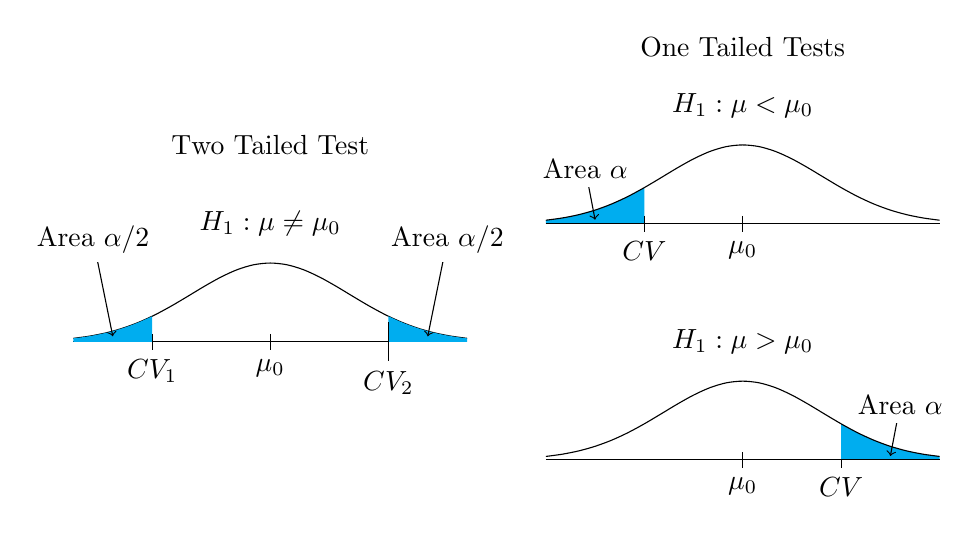
\begin{tikzpicture}

\node at (-3, 2.5) {Two Tailed Test};
\node at (-3, 1.5) {$H_1: \mu \neq \mu_0$};
\draw (-5.5, 0) -- (-0.5, 0);
\draw[domain=-2.5:2.5, smooth, variable=\x] plot ({\x - 3)}, {exp(-0.5 * \x * \x)});
\draw (-3, 0.10) -- (-3, -0.10) node[below] {$\mu_0$};

\fill[cyan, domain=-2.5:-1.5, variable=\x] (-5.5, 0) -- plot ({\x - 3},  {exp(-0.5 * \x * \x)}) -- (-4.5, 0) -- cycle;
\draw (-4.5, 0.10) -- (-4.5, -0.10) node[below] {$CV_1$};

\fill[cyan, domain=1.5:2.5, variable=\x] (-1.5, 0) -- plot ({\x - 3},  {exp(-0.5 * \x * \x)}) -- (-0.5, 0) -- cycle;
\draw (-1.5, 0.25) -- (-1.5, -0.25) node[below] {$CV_2$};


\draw[<-] (-1, 0.07) -- (-0.75, 1.3) node[fill = white] {Area $\alpha/2$};
\draw[<-] (-5, 0.07) -- (-5.25, 1.3) node[fill = white] {Area $\alpha/2$};

\node at (3, 3.75) {One Tailed Tests};

\node at (3, 3) {$H_1: \mu < \mu_0$};
\fill[cyan, domain=-2.5:-1.25, variable=\x] (0.5, 1.5) -- plot ({\x + 3},  {exp(-0.5 * \x * \x) + 1.5}) -- (1.75, 1.5) -- cycle;
\draw[domain=-2.5:2.5, smooth, variable=\x] plot ({\x + 3)}, {exp(-0.5 * \x * \x) + 1.5});
\draw (0.5, 1.5) -- (5.5, 1.5);
\draw (3, 1.6) -- (3, 1.4) node[below] {$\mu_0$};
\draw[<-] (1.125, 1.55) -- (1, 2.2) node[fill = white] {Area $\alpha$};

\draw (1.75, 1.60) -- (1.75, 1.4) node[below] {$CV$};

\node at (3, 0) {$H_1: \mu > \mu_0$};

\fill[cyan, domain=1.25:2.5, variable=\x] (4.25, -1.5) -- plot ({\x + 3},  {exp(-0.5 * \x * \x) - 1.5}) -- (5.5, -1.5) -- cycle;
\draw[domain=-2.5:2.5, smooth, variable=\x] plot ({\x + 3)}, {exp(-0.5 * \x * \x) - 1.5}); 
\draw (3, -1.4) -- (3, -1.6) node[below] {$\mu_0$};
 \draw (0.5, -1.5) -- (5.5, -1.5);
 \draw (4.25, -1.5) -- (4.25, -1.6) node[below] {$CV$};
\draw[<-] (4.875, -1.45) -- (5, -0.8) node[fill = white] {Area $\alpha$}; 

  
\end{tikzpicture}


\end{frame}

\begin{frame}
\frametitle{Compute the Test Statistic}
\begin{Definition}
A {\bf test statistic} quantifies the observed data in a way that would distinguish the null from the alternative hypothesis.
\end{Definition}

\end{frame}

\begin{frame}
\frametitle{Make a Decision}
\begin{Definition}
The $\boldsymbol p${\bf -value} is the probability of an observation being at least as extreme as the test statistic assuming the null hypothesis is true.
\end{Definition}

\end{frame}

\begin{frame}
\frametitle{Make a Decision Cont.}
\begin{itemize}
\item If the $p$-value is greater than or equal to $\alpha$, we {\it fail to reject the null hypothesis}.
\item If the $p$-value is less than $\alpha$, we {\it reject the null hypothesis}.
\end{itemize}
\end{frame}

\begin{frame}
\frametitle{Types of Error}
\begin{center}
\begin{tabular}{ c | c | c c }
							&						&	\multicolumn{2}{c}{Decision}		\\ \hline
							&						&	Fail to Reject Null	&	Reject Null	\\\hline
\multirow{4}{*}{Ground Truth}		&	\multirow{2}{*}{Null True}	&	Correct			&	Type I Error	\\
							&						&	$1 - \alpha$		&	$\alpha$		\\
							&	\multirow{2}{*}{Null False}	&	Type II Error		&	Correct		\\
							&						&	$\beta$			&	$1 - \beta$	\\		
\end{tabular}
\end{center}

\end{frame}

\begin{frame}
\frametitle{Confidence and Power}
\begin{Definition}
\begin{itemize}
\item The {\bf confidence level} is $1-\alpha$.
\item The {\bf power} is $1 - \beta$.
\end{itemize}
\end{Definition}
\end{frame}


\begin{frame}
\frametitle{Types of Hypothesis Tests}
\small
Incomplete list of types of hypothesis tests.

\begin{tabular}{p{1.3in} c p{2in}}
\hline
Name				&	Test Statistic							&	Comments \\\hline
One-sample $z$-test		&	$z = \frac{\bar{X} - \mu_0}{\sigma/\sqrt{n}}$	&	\tiny Normal population or large $n$ and known $\sigma$. The value $\mu_0$ is the mean assuming the null hypothesis. \\
One-sample $t$-test		&	$t = \frac{\bar{x} - \mu_0}{s/\sqrt{n}}$			&	\tiny Normal population or large $n$ and unknown $\sigma$. The degrees of freedom are $df = n - 1$\\
One-proportion $z$-test	&	$z = \frac{\hat{p} - p_0}{\sqrt{\frac{p_0(1 - p_0)}{n}}}$& \tiny	$p_0$ is the proportion under the null hypothesis and $\min\{ n\cdot p_0, n\cdot (1- p_0)\} > 10$\\
\end{tabular}
\end{frame}

\begin{frame}
\frametitle{Notation}

\begin{tabular}{l | c c c}
					&	{\bf Population}					&	{\bf Sample}\\\hline
{\bf Mean}				&	$\mu = E[X]$					&	$\bar{x} = \displaystyle\frac{1}{n}\sum_{k = 1}^n x_k$\\
{\bf Variance}			&	$\sigma^2 = E[(X - \mu)^2]$		&	$s^2 = \displaystyle\frac{1}{n - 1}\sum_{k = 1}^n (x_k - \bar{x})^2$\\
{\bf Standard Deviation}	&	$\sigma = \sqrt{E[(X - \mu)^2]}$		&	$s = \sqrt{ \displaystyle\frac{1}{n - 1}\sum_{k = 1}^n (x_k - \bar{x})^2}$\\
\end{tabular}

\end{frame}

\begin{frame}
\frametitle{Sample Standard Deviation}

$$s = \sqrt{\frac{1}{n - 1}\sum_{k = 1}^n (x_k - \bar{x})^2}$$

\end{frame}

\begin{frame}[fragile]
\frametitle{Sample Standard Deviation Example}
\small 
\begin{Example}
Find the distribution of the biased and unbiased standard deviation when ten elements are sampled from $\mathcal{N}(0, 1^2)$.
\end{Example}

{\bf Solution.}
{
\linespread{0.8}
\tiny
\begin{verbatim*}
# Import modules
import numpy as np, matplotlib.pyplot as plt
from scipy.stats import norm

# Use latex
plt.rcParams['text.usetex'] = True

# Use Seaborn style
plt.style.use('seaborn')

# Set random seed
np.random.seed(0)

# Define number of trials
trials = 10000

# Generate normal rvs with mean 0 and variance 1
Z = norm.rvs(loc = 0, scale = 1, size = (trials, 10))

# Calculate the sd without bias correction
sd0 = np.apply_along_axis(lambda arr: np.std(arr, ddof = 0), 1, Z)

# Calculate the sd with bias correction
sd1 = np.apply_along_axis(lambda arr: np.std(arr, ddof = 1), 1, Z)
\end{verbatim*}
 }


\end{frame}

\begin{frame}[fragile]
\frametitle{Sample Standard Deviation Example Cont.}
{
\linespread{0.8}
\tiny
\begin{verbatim*}
# Set up subplots
fig, ax = plt.subplots(1, 2, sharex = True, sharey = True, figsize = (15, 5))

ax[0].hist(sd0, bins = int(np.sqrt(trials)), density = True)
ax[0].axvline(x = 1, color = 'red', label = 'True')
ax[0].axvline(x = np.mean(sd0), color = 'orange', label = 'Mean SD')

ax[0].legend()
ax[0].title.set_text(r'$\displaystyle\sqrt{\frac{1}{n}\sum_{k = 1}^n (x_k - \bar{x})^2}$')

ax[1].hist(sd1, bins = int(np.sqrt(trials)), density = True)
ax[1].axvline(x = 1, color = 'red', label = 'True')
ax[1].axvline(x = np.mean(sd1), color = 'orange', label = 'Mean SD')

ax[1].legend()
ax[1].title.set_text(r'$\displaystyle\sqrt{\frac{1}{n - 1}\sum_{k = 1}^n (x_k - \bar{x})^2}$')

# Give entire figure title
fig.suptitle('Standard Deviation with and without Bias Correction')

# Add padding
fig.tight_layout(pad = 1)

# Save the figure
plt.savefig(r'[location on machine]')

plt.show()
\end{verbatim*}
 }

\end{frame}

\begin{frame}[fragile]
\frametitle{Sample Standard Deviation Example Result}
\begin{center}
\includegraphics[scale = 0.3]{ex14.png}
\end{center}
\end{frame}

\begin{frame}
\frametitle{Student's $\boldsymbol t$-Distribution}
\begin{Definition}
Let $x_1, x_2,\ldots x_n\sim{\mathcal{N}(\mu, \sigma^2)}$ be independent and identically distributed samples. Then
$$
T = \frac{\bar{x} - \mu}{s/\sqrt{n}}
$$
follows a $t$-distribution with $n-1$ degrees of freedom. We often write $T \sim{t_{n-1}}$.
\end{Definition}
For $n > 30$ the $t$-distribution is approximately equal to a normal distribution. As a result, this distribution is only relevant for small samples. 
\end{frame}

\begin{frame}[t]
\frametitle{Hypothesis Testing with Unknown Variance}
\tiny
\begin{Example}
You sample the numbers 8, 0.5, 0, and $-0.5$ from a normal distribution. Perform a hypothesis test to determine whether the mean of the distribution is larger than 0 at a significance level of 10\%. Note: If $T\sim{t_3}$, then $P(T > 1.638) \approx 10\%$.
\end{Example}

\end{frame}

\begin{frame}[t]
\frametitle{Hypothesis Testing Proportions}
\tiny
\begin{Example}
You flip a coin 100 times and it lands heads 65 times. Perform a hypothesis test to determine whether the probability of landing heads is statistically different from 50\% at a 95\% confidence level.
\end{Example}


\end{frame}

\begin{frame}
\frametitle{Confidence Interval}
The population parameter lies in this interval with probability $1 - \alpha$.
\begin{itemize}
\item Known Variance: 
$$
\left(\bar{x} - z_{\alpha/2} \frac{\sigma}{\sqrt{n}}, \bar{x} + z_{1 - \alpha/2} \frac{\sigma}{\sqrt{n}}\right).
$$
\item Unknown Variance: 
$$
\left(\bar{x} - t_{\alpha/2} \frac{s}{\sqrt{n}}, \bar{x} + t_{1 - \alpha/2} \frac{s}{\sqrt{n}}\right).
$$ 
Degrees of freedom are $n-1$.
\item Proportion: 
$$
\left(\hat{p} - z_{\alpha/2}\sqrt{\frac{\hat{p}(1 - \hat{p})}{n}}, \hat{p} + z_{1 - \alpha/2} \sqrt{\frac{\hat{p}(1 - \hat{p})}{n}}\right).
$$
\end{itemize}
\end{frame}


\end{document}